\documentclass{article}

\usepackage[utf8]{inputenc}
\usepackage[margin=2cm]{geometry}
\usepackage{multicol}
\usepackage{color}
\usepackage{float}
\usepackage{graphicx}
\graphicspath{{images/navigation/}{images/app/}{images/overview/}}

\title{Software Design Study Report}
\author{A-Team}

\begin{document}
\maketitle

%\begin{multicols}{2}
\begin{abstract}
  Cars are ubiquitous in our modern lifestyles, unfortunately, the software systems in them do not keep up with other computing systems that we use. In this report, we aim to show how we tackled the problems and areas for improvement that we found in current car systems. Five areas of a modern car's feature set were focused on weekly, these being; the dashboard, media, navigation, safety and an accompanying smartphone app.
\end{abstract}

\section*{Introduction}
For years car companies have invested relatively little into their car's information systems and technological abilities. Inbuilt Sat Nav systems are often hard to use, update and are counter-intuitive. Since car companies are slow to adopt new technologies, even features that would have been possible many many years ago have not been widely used yet. For example, we still use the physical dials in the instrument cluster that we have used for years.

We have created an attractive and modern solution for digital technology in a car that we hope to see in future modern cars in production. In Section~\ref{sec:system-design} we will give explain the technical elements of our system design that can be found ranging from navigation to safety features. In Section~\ref{sec:nav} we will go into detail on the design process of our navigation system. In Section~\ref{sec:app} we will go into detail on the design process of our accompanying smartphone app.

\section{Overall system design}\label{sec:system-design}
\subsection{Algorithms}\label{ssec:algorithms}
\begin{itemize}
  \item Bidirectional A* Algorithm
    \begin{itemize}
      \item Heuristics
        % Talk about
    \end{itemize}
  \item K means algorithm --- grouping convoys
  \item Learning algorithm --- user preferences, Contextually Aware Routing etc
    % FIND A LEARNING ALGORITHM
  \item Safety Detection algorithms
    \begin{itemize}
      \item Head pose algorithm
      \item Tesla radar system?
      \item Recognising bikes --- trained from training images which are bikes with riders
        % This is if we are detecting bikes using this method of detecting bikes (we mentioned using the 360 degree vision from the cameras for seeing bikes)
    \end{itemize}
  \item Something for tiredness detection
\end{itemize}

\subsection{Storage}\label{ssec:storage} % Chris
Our design has three places that data will be stored, some data being temporary and some persistent. We will store information in the cloud, in the car's local SSD storage and on users of the app's smartphones.

The cloud will be used for the majority of storage, it is where persistent data will be synchronised to from the phone app and car. Storage for most data such as user profiles will be kept in an encrypted Oracle database. The cloud will store user profiles that contain details such as saved routes, privileges, seat preferences, dashboard layout, contacts and driver stats. The cloud will also store details about convoy groups, containing data on members, member locations, group messages, routes etc. Since the cloud hosts the API used by the car and app, other miscellaneous data will also be stored here such as software updates.

The car's internal SSD storage will be used for fast reading and writing of synchronised files and cached data primarily. Data queried from the cloud will be cached to grant a more seamless experience even when the car is not connected to the internet. Examples of cached data from the cloud include favourite routes, dashboard layout and seat positions. Since the centre console system is built around the Android platform, we have been able to easily allow certain apps from the Play Store. One example of an app that we would allow on the system is Spotify, for music playback. The Spotify app will be able to store all of its settings, cached data and offline playlists in the car's internal storage as well. Local music files synchronised from a home network will be stored in the car's internal storage. The dashcams will also record their video to the internal storage of the car, this will be limited to a default percentage of the drive's capacity (SSD can be upgraded) and recordings will overwrite old footage in order to reuse the assigned storage space. The basic version of the system will likely have a 120GB SSD, however, this could easily be upgraded by swapping out the drive from the glove box.

The accompanying car smartphone app does not require much storage at all since it must be connected to the internet or car to make any changes. Data from the cloud, car and app will be cached so that it may still be accessible for short connectivity outages.

\subsection{Data Structures}\label{ssec:data-structures} % Chris
In the system that we have designed, we require a few different data structures in order make our system efficient and easy to work with.

For our navigation algorithm, we decided to model the street map as a graph. Road junctions, route starting point and route destination are all represented as nodes in the graph, with roads being the edges that connect the nodes of the graph. This graph structure is most appropriate for us to use in our bidirectional A* search algorithm.

Routes will be kept in a JSON format with a JSON object containing two lists, one list containing nodes IDs of a route and the other containing the edge IDs. List items will be in chronological order for the route. The system is able to present the route on-screen by reading the lists to build the section of the street map graph that represents the route. This JSON format also allows for sections of the route to be updated easily by swapping out and adding nodes and edges. Another benefit of this format is that it is easy to implement the transferring of these routes from the app to the car.

The customisable dashboard layout will also be stored in a JSON format with widgets stored in a list object and more general details in a separate object. Widget objects in the list contain information about their relative position, size and styling in the dashboard.

User profile data such as username, route preferences etc.\ will all be kept in an encrypted Oracle database in the cloud, this will allow for us to have granular control over what information we receive when requesting user information.

An SQLite database will exist in the local storage of the car, this database will contain details of local music files that are also stored in the car's local storage. Music files that have been added to the car will have their song, album and artist names looked up and stored in the database. The SQLite database provides access to song details to the centre console and car app.

The smartphone app for the car system will use the same data structure for maps as the car uses. Cache data from the cloud and car will be stored in an SQLite database.

\subsection{User Accounts --- Matt}\label{ssec:user-accounts}
Something that we found is lacking across intelligent car systems in the market is the use of portable user profiles. By this we mean profiles that can be used across several cars, applying user settings and preferences where applicable.
There are several ways in which such data can be encapsulated and moved from car to car, including serving a database from a server to the car, transport via Bluetooth directly from a smartphone, use of NFC tags and many others.
\subsubsection{Storage and transport}
The method we found most suitable for doing this works by storing the data relative to each user profile online in an SQLite database and then serving it either directly to the car when a user logs in from in-car interfaces or to a smartphone application. Following this, the user is able to transfer the data to the car via Bluetooth with the press of a button. The data is cached on the phone and car, as applicable, to allow access even when internet access is limited or not available.
\subsubsection{Cardinality of accounts, vehicles and shared data}
Each user will have one account that will be able to contain multiple car profiles. Car profiles can share generic information, such as preferences regarding routing, music, favourite temperatures, speed dial contacts, etcetera if the user specifies so. Information specific to the car make and model, such as steering rack height, seat adjustments, wing mirror adjustments shall stay bonded to each car profile.
\begin{figure}[H]
  \centering
  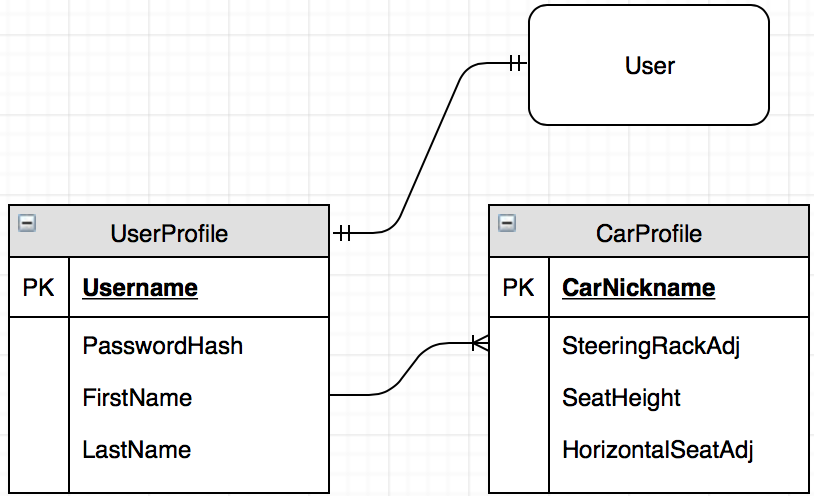
\includegraphics[scale=0.7]{profile-cardinality}
  \caption{Visualisation of cardinality of user profiles}\label{cardinality}
\end{figure}


\subsection{Communications \& Data Flows --- Tyler}\label{ssec:communications-data}
Within our system, we have communications between the Mobile App, the Car and our Cloud, with links to external APIs.

\subsubsection{Communication between car and cloud}
The car and the cloud communicate with each other mainly to synchronise information. The car sends hashes and timestamps of its files to the server, which compares them with the latest versions. The files which are different are sent back to the car for synchronisation.

There will be multiple streams of live data going between the cloud and the car continuously. This will consist of navigation updates, API calls and streaming of the cars camera feeds.
During navigation in convoys, the cars location is sent to the cloud and the associated group member's locations are pulled down from the cloud. This is so the location of other group members is regularly updated on the navigation display.
%Live streaming footage of the cars camera feeds are sent to the cloud over RTSP -- is this through the cloud or straight to phone?

Since the car and the mobile app can both change user profile settings, this will 

All the system updates for the car's software will be downloaded through the cloud. 

The cloud will always be listening for real time event data. For example if 

\begin{itemize}
  \item Hashes and timestamps are compared on the server to decide what to synchronise
  \item Synchronisation with user profiles
  \item System updates
  \item Map updates
  \begin{itemize}
    \item Convoy information
  \end{itemize}
  \item Streaming camera feeds
  \item API calls to the cloud
  \item Real time event data, for example someone is breaking into your car, car stats (warning lights)
\end{itemize}
\subsubsection{Communication between car and phone}
Communications between the car and the phone consist of initial connection, instructions and data transfer. Establishing a connection is done by pairing the phone to the car by means of NFC, this will authenticate the phone with the car for communications over Bluetooth and Wi-Fi. Authentication can also be achieved by typical manual methods such as typing in a password. There will also be the standard Bluetooth communication between the phone and the car such as sharing contacts and taking calls.

Many features of the app rely on communication with the car in order for them to work. These messages are sent between the phone to the car's central computing unit to be processed. Features which send instructions to the car to control the car's hardware have two different types of communication.

Firstly, instructions such as turn the heating on or toggling headlights will be a be on an on/off basis. For example setting the temperature to 20 degrees will keep it at that until it has changed.

Secondly, instruction-critical tasks such as remote controlling the car with the phone app, rapidly send instructions to the car to ensure the car is performing actions safely and as the user expects. For example, if a user is holding the steering wheel at a 45 degree angle, the associated instruction will be sent constantly and processed by the central computing unit until the user changes the rotation. If the phone would happen to lose connection and the instructions stop being received by the car, the car is stopped.

Features for controlling music within the car are communicated over Wi-Fi and Bluetooth. The local music library of the car is synced with the phone, and also there is a Spotify account linked to the drivers user profile. Which is logged in on the centre console.

All messages regarding the control of music with the app, are encapsulated within a JSON object. These messages will hold instructions such as play, pause and song requests. Song requests will contain music file names and the library they are stored in.
If music is from Spotify, then associated actions for controlling the Spotify account, which is logged in on the centre console are embedded within the message.

There is also the option to control the centre console Spotify account using Spotify's ``Spotify connect'' service. This allows you to control other Spotify devices on the same network. The Wi-Fi network of the car in this case.

\subsubsection{Communication between phone and cloud}

\begin{itemize}
  \item Hashes and timestamps are compared on the server to decide what to synchronise
  \item API calls to the cloud
  \item Car camera feeds can be streamed to the phone on-demand over RTSP
  \item Information regarding convoy setup on phone
  \item Car software updates from cloud (Gives ability to update car with phone)
  \item Real time event data from cloud eg someone breaking into your car, car stats (warning lights)
\end{itemize}
\subsubsection{Communication between car and external APIs}
% Talk about how it connects to the cloud which provides a link to the APIs
\begin{itemize}
  \item Roadworks
  \item Traffic
  \item Weather
  \item Public Transport
  \item Note: All API calls are relative to the country the car is located in.
\end{itemize}

\subsection{Information Security --- Joe}\label{ssec:information-security}
A major focus for any internet connected technology is security, and with our car systems it is no different- the last thing a customer would want is to have their car stolen by it being driven into the distance by a remote thief. We employ a model of `encryption everywhere' to ensure maximum data security. Security is a primary focus in every aspect of the car system, the following non-exhaustive list are some of our main focuses

\subsubsection{Data communication}
Every connection that is made in our ecosystem leverages the flexibility and security of TLS for both encryption and authentication. TLS provides a strong suite of ciphers cross-compatible with any device. Industry standard hardening techniques are employed at both client and server end to ensure the strongest connection possible such as only using strong mutually-agreed cipher suites and key exchanges.

This widespread usage of full transport encryption is viable due to the hardware-accelerated AES-NI and similar instruction sets built into most modern CPUs by manufacturers like Intel, AMD and ARM* (dependent on model and chip manufacturer). Without hardware support, encryption would be very expensive in terms of computation for every device: servers, cars and most importantly mobile devices such as smartphones and embedded devices.

Performing AES or similar encryption purely in software is very slow and consumes a significant amount of CPU cycles and battery power resulting in a poor experience and making encryption on lower power and mobile devices not at all feasible.

Another advantage of using TLS is `Perfect Forward Secrecy' of data when the appropriate key-exchange protocol is used such as a Diffe-Hellman based exchange method. This provides the guarantee that any data that is intercepted in transport by a 3rd party cannot decrypt the data with a previously apprehended pre-shared key or certificate as the short-lived session token has been lost.

\subsubsection{Data storage \& encryption}
{\Large\color{red} Decide data storage encryption}

\subsubsection{User authentication}


\subsubsection{???}
\subsubsection{Profit}



\begin{itemize}
  \item Database encryption in the cloud
    % * <frebib@gmail.com> 2017-03-20T22:31:12.891Z:
    %
    % Is this a thing?
    % Maybe the data can use end-to-end encryption, only unlockable with a key from the user account?
    % ^ That however means the user is fleeced if they forget their password
    %
    % ^.
  \item HTTPS for all internet communications
  \item WPA2-PSK with AES for Wi-Fi hotspot login
  \item X.509 certificate for the car
\end{itemize}

\subsection{Interaction Design --- Matt}\label{ssec:interaction-design}
The interaction designs used on our product's interfaces were designed loosely based on designs from industry leading companies but tailored to integrate our ideas and implement some recurrent suggestions found throughout our research, which has seen over 100 responses. Our product requires three main interactive interfaces for users to effectively communicate with the in-car system:

\subsubsection{Centre console}\label{sssec:centre-console}
This is a 10 inch screen located in the middle section of the dashboard. Its purpose is that of displaying most of the information that flows through the car that may be of interest to the user and for the user to interact with it. For instance, destination input for the navigation system, joining and managing convoys, customising the instrument cluster, querying the system for detailed engine data and many more interactions will be performed on this device.

We found that in the recent years the integration of touch screens on dashboards has become a recurrent trend amongst major manufacturers and believe that it is an essential feature for the cars of the future due to how visible, versatile and aesthetically pleasing they are.

\subsubsection{Mobile app}\label{sssec:mobile-app}
As usage of mobile apps is constantly increasing, more and more industry leading companies are adopting this as a new mean of interaction with their automobiles. We firmly believe that this will become and essential feature to all cars within a few year and therefore have designed and prototyped one. More detail can be found in Section~\ref{sec:app}.

\subsubsection{Device on rear doors}\label{sssec:device-rear-doors}
Each of the rear door cards will be fitted with a 5 inch touch screen device that enables passengers in the rear of the car to search and add songs to the cars' shared music queue from different streaming services or a local library.

\subsection{Aesthetics/Graphical Design --- Matt}\label{ssec:aesthetics}
% User Interfaces of the above devices
An effort was made to follow current styling standards used in industry to give the user a familiar experience, therefore flat designs were used where possible. Also characterising our design are large icons and avoidance of large swathes of text.

\subsubsection{Dashboard cluster screen}\label{sssec:cluster-screen}
A screen will be replacing the usual instrument cluster behind the steering wheel. This will display information relative to speed, engine revolutions, fuel levels as it has been doing for the past decades but with the twist

%%%%%%%%%%%%%%%%%%%%%
%	PLAN
%%%%%%%%%%%%%%%%%%%%%
\begin{itemize}
  \item Centre console
  \item Smaller navigation console above centre console
  \item Mobile phone
  \item Rear side door device
    % Justifications of why we have chosen these designs
\end{itemize}




%%%%%%%%%%%%%%
%
%	NAV
%
%%%%%%%%%%%%%%
\section{Feature 1: Navigation}\label{sec:nav}

\subsection{Research --- Lewis}\label{ssec:nav-research}
As part of the brainstorming process, we investigated current technology to see how the current navigation systems were perceived by various people. The first part of this research takes the form of a questionnaire we created to gain opinions on both current technology and some of our ideas. From this, we confirmed our beliefs that most people use their phone as their SatNav device; and are generally happy with current methods of controlling a SatNav, being touch screen and voice control. We also gained some insight into some design decisions to take, with a majority of survey participants being interested in seeing friends travelling with them; speed cameras; traffic; and road obstacles such as roadworks, accidents and breakdowns, on the map - while there was less interest in tracking emergency vehicles and breakdown recovery vehicles. There is also a high amount of interest in having various destination suggestions available to the driver. The survey  indicated to us that some features are already being executed well; most people find the directions given by their SatNav to be quite clear.
% Link to survey responses?

We also conducted 
\begin{itemize}
  \item Questionnaires
  \item Researching latest technology
\end{itemize}

\subsection{Brainstorming --- Matt}\label{ssec:nav-brainstorming}
% Should we cite our initial ideas document?
In the first stage of our brainstorming we created a Google document which allowed us to collaboratively write down all the ideas we could come up with. By discussing them within our group, new ideas kept being generated and even different variations of the ideas we already had. In order to keep the design space as open as possible, during this stage, all ideas were noted down and considered, no matter how far fetched. Following the initial stage, and an iteration of research, we went through the document and filtered it, as a group, for the concepts that we wanted to take forward in our design. During the second stage of brainstorming we created a new document, containing only the chosen ideas to expand and research them in more depth.

An aid we found very useful was personas, a list of made-up personalities with realistic interests, jobs and attributes. During the brainstorming each of us tried to empathise with the different personas and think about their habits, things they enjoy, their mental states throughout different times of the day and from there, think of their needs, features they would enjoy and why.

Some of the ideas that came from our brainstorm are: Convoy tracking using K-Means clustering, public transport integration (including park and ride suggestions), route scheduling via either mobile app or in-car interfaces.

\subsection{Tech background --- Lewis}\label{ssec:nav-tech}
(Most of this seems like it would be algorithms again, so we plan to expand on the algorithms further than was detailed in section 2.1)
\begin{itemize}
  \item Bidirectional A* search
  \item K-means clustering
\end{itemize}

\subsection{Convoy}\label{ssec:nav-convoy} % Chris
Convoys are a feature in our system, designed to allow a party to all route to the same destination, tracking members and having functionality for scheduled stops, rerouting and group calls. From the navigation menu, the user can select to either set up or join a convoy. The user that chooses to set up a convoy is given a six-digit code that they can then share via social media or any other way. Users that choose to join the convoy must enter the six digit code they were given by the convoy creator. The convoy creator is able to set the route destination, any stop off points and optionally give the convoy a name.

Once a convoy is set up, members of the convoy are able to see the shared route and coloured icons for members on the map. In the case that convoy members are starting their journey from different places, members will be grouped, with groups having different routes to a point of convergence. Like the normal navigation mode in our system, the route for an individual can be adjusted to re-route them back to the convoy in the case that they go the wrong way. Another feature of the convoy system is that it provides the ability to make group VoIP calls so that users can communicate hands-free, this is done using peer-to-peer technology over the car's internet connection (provided it has one).

Users may want to use convoys despite being far apart from each other, in this case, users may not be likely to arrive at similar times and so routes are individually calculated on each car's system and uploaded to the cloud. Each user follows their own route and can see the expected time of arrival for other members in a sidebar. Should two routes converge at any point, members will be moved onto a shared route when they reach that point, making meeting up more likely and reducing the number of routes to be stored in the cloud.

A convoy member can leave the convoy at any time, however, there are points at which the system will prompt them to leave the convoy. The first occasion for a prompt is when the current driver of the car changes, the new driver might be wanting to travel to somewhere else. The driver can, of course, cancel the prompt, this is useful for a situation where for example people share the responsibility of the driving for a long journey. Another time that a prompt to leave a convoy may occur is in the event that all convoy members have arrived at the destination, at this point, there will typically be no further use for the convoy. The final situation for a prompt to leave a convoy is if the car is inactive for 24 hours, users typically will not be resuming a group journey after such a long time.

Convoy data is collected and distributed to all convoy members from the cloud. The cars will download routes via the cloud API and send GPS location updates to the cloud every few seconds, these location updates will then be pinged to all other convoy members to keep the location of cars synchronised on all screens. Once the cloud receives a new location for a member, it immediately deletes the old, redundant location.

Limited functionality of the convoys feature is available through the app. Users with the app are able to set up or join a convoy, this data is synchronised to the cloud and then used by the car.

There are of course limitations to this feature. Convoys require an internet connection to update member locations. If any member fails to update their location, their icon will stay in place and fade away until a connection is regained and the location is updated once again.

\subsection{Design choices \& argumentation --- Lewis}\label{ssec:nav-design}
\begin{itemize}
  \item QOC
  \item Justification for algorithms
    % Would this be better placed in the previous section?
    \begin{itemize}
      \item Routing
      \item Clustering
    \end{itemize}
\end{itemize}

\subsection{Prototypes \& user testing}\label{ssec:nav-prototypes-testing}
\begin{itemize}
  \item Lo-Fi and Hi-Fi prototypes of Navigation and Convoy
\end{itemize}

\subsection{Final design}\label{ssec:nav-final-design}

\subsection{Evaluation \& how it fits into whole system}\label{ssec:nav-evaluation}




%%%%%%%%%%%%%%
%
%	APP
%
%%%%%%%%%%%%%%
\section{Feature 2: App}\label{sec:app}

\subsection{Research --- Matt}\label{ssec:app-research}
Research and brainstorming were conducted in a cyclic manner to ensure that the latest technologies relevant to this sector of the automotive industry were taken into consideration. Extensive research revealed that most leading companies such as Jaguar, BMW and Tesla already offer multi-platform mobile apps that compliment their automobiles. Each of the above boasts at least one of the features that we intended to integrate into our systems such as remote control and seamless route porting from smartphone to car. From brainstorming through to coding the prototype, our focus was directed on how to improve on existing products and also integrate our novel features.
The research methods we used included a questionnaire, installing and using manufacturers apps on our mobile devices, browsing their websites and reading through papers and articles found through numerous searches on search engines.
\begin{itemize}
  \item Existing apps that accompany a car
  \item Current technology
  \item How personas might want to interact with an app
    % Link to a persona document in the appendix
\end{itemize}
\subsection{Brainstorming --- Chris}\label{ssec:app-brainstorming}

\begin{itemize}
  % First 3 points are same as section 3.2
  \item Collectively worked together to put down all of our ideas into a Google doc
  \item No ruling out of ideas
  \item Finally moved everything into a final document. Discussed each point as a group to decide what was worth expanding
  \item Things specific to the app brainstorm i.e.\ the ideas to come out of it
\end{itemize}
\subsection{Tech background --- Tyler}\label{ssec:app-tech}
\begin{itemize}
  \item Communication
    \begin{itemize}
      \item (See section 2.4?)
      \item To and from car
        \begin{itemize}
          \item Initial connection with the car (Bluetooth/Wi-Fi/RFID)
          \item Communicating remote control instructions
          \item Other instructions (Media control, Controlling hardware)
        \end{itemize}
      \item To and from Cloud
        \begin{itemize}
          \item Authenticating User profiles
          \item Syncing data
          \item Feeds which are streamed (Camera feeds)
          \item Information such as Car location
        \end{itemize}
    \end{itemize}
\end{itemize}
% Repeating what is said in communication (2.4) ^^

\subsection{Design choices \& argumentation --- Lewis (maybe)}\label{ssec:app-design}
\begin{itemize}
  \item QOC (to be made)
\end{itemize}

\subsection{Prototypes \& user testing}\label{ssec:app-prototypes-testing}
\begin{figure}[H]
  \centering
  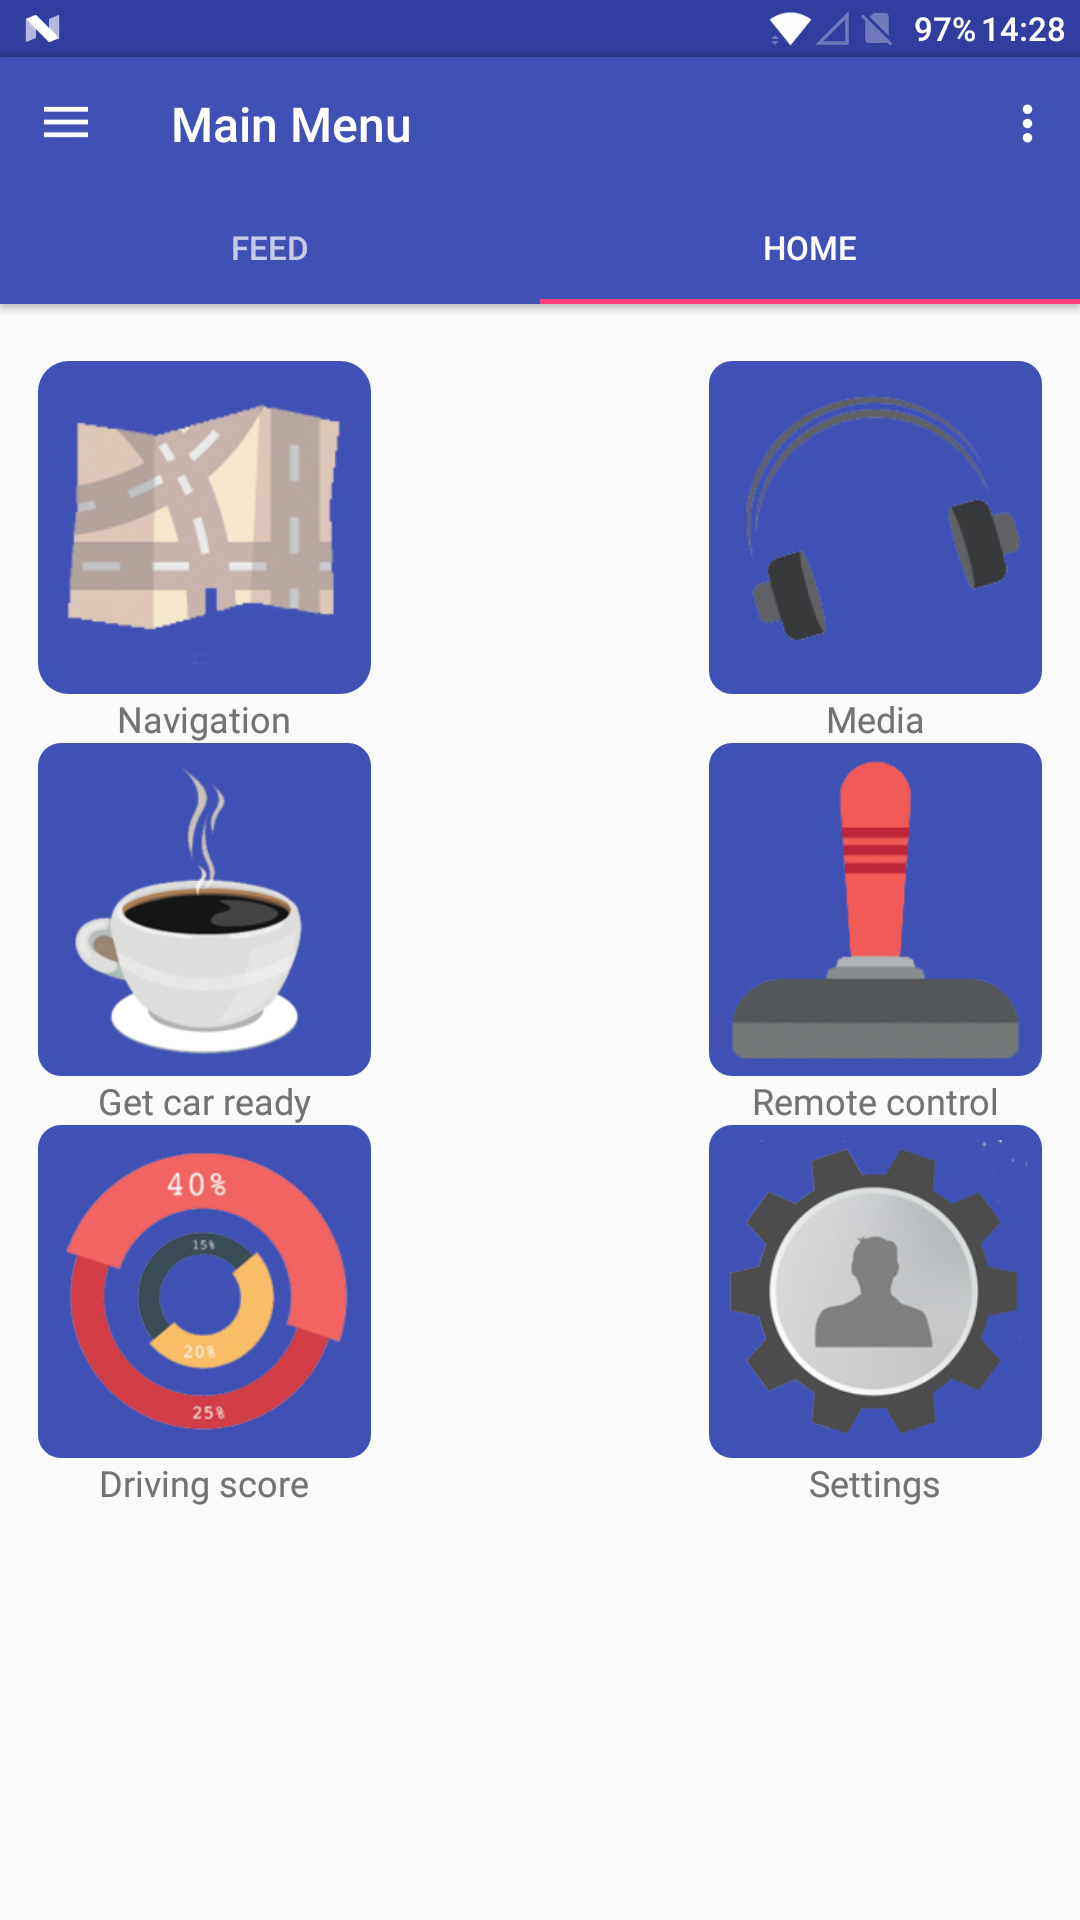
\includegraphics[scale=0.25]{main-menu}
  \caption{Hi-Fi prototype of app main menu.}\label{main-menu}
\end{figure}

\subsection{Final design}\label{ssec:app-final-design}

\subsection{Evaluation \& how it fits into whole system}\label{ssec:app-evaluation}

\section{Other areas}\label{sec:other}

Annotate slides on changes we would make going forwards
\section{References}\label{sec:references}

%\end{multicols}

\end{document}

% vim: set tabstop=2 shiftwidth=2:
